%%%%%%%%%%%%%%%%%%%%%%%%%%%%%%%%%%%%%%%%%
% Tufte-Style Book (Minimal Template)
% LaTeX Template
% Version 1.0 (5/1/13)
%
% This template has been downloaded from:
% http://www.LaTeXTemplates.com
%
% License:
% CC BY-NC-SA 3.0 (http://creativecommons.org/licenses/by-nc-sa/3.0/)
%
% IMPORTANT NOTE:
% In addition to running BibTeX to compile the reference list from the .bib
% file, you will need to run MakeIndex to compile the index at the end of the
% document.
%
%%%%%%%%%%%%%%%%%%%%%%%%%%%%%%%%%%%%%%%%%

%----------------------------------------------------------------------------------------
%	PACKAGES AND OTHER DOCUMENT CONFIGURATIONS
%----------------------------------------------------------------------------------------

\documentclass{tufte-book} % Use the tufte-book class which in turn uses the tufte-common class

\makeatletter
% Paragraph indentation and separation for normal text
\renewcommand{\@tufte@reset@par}{%
  \setlength{\RaggedRightParindent}{0pc}%
  \setlength{\JustifyingParindent}{0pc}%
  \setlength{\parindent}{0pc}%
  \setlength{\parskip}{10pt}%
}
\@tufte@reset@par

% Paragraph indentation and separation for marginal text
\renewcommand{\@tufte@margin@par}{%
  \setlength{\RaggedRightParindent}{0pc}%
  \setlength{\JustifyingParindent}{0pc}%
  \setlength{\parindent}{0pc}%
  \setlength{\parskip}{10pt}%
}
\makeatother
  
\usepackage{ifxetex}
\ifxetex
  \newcommand{\textlspace}[2][5]{%
    \begingroup\addfontfeatures{LetterSpace=#1}#2\endgroup
  }
  \renewcommand{\allcapsspacing}[1]{\textlspace[15]{#1}}
  \renewcommand{\smallcapsspacing}[1]{\textlspace[10]{#1}}
  \renewcommand{\allcaps}[1]{\textlspace[15]{\MakeTextUppercase{#1}}}
  \renewcommand{\smallcaps}[1]{\smallcapsspacing{\scshape\MakeTextLowercase{#1}}}
  \renewcommand{\textsc}[1]{\smallcapsspacing{\textsmallcaps{#1}}}
  \usepackage{fontspec}
\fi
  
\hypersetup{colorlinks} % Comment this line if you don't wish to have colored links

\usepackage{microtype} % Improves character and word spacing

\usepackage{lipsum} % Inserts dummy text

\usepackage{booktabs} % Better horizontal rules in tables

\usepackage{graphicx} % Needed to insert images into the document
\graphicspath{{graphics/}} % Sets the default location of pictures
\setkeys{Gin}{width=\linewidth,totalheight=\textheight,keepaspectratio} % Improves figure scaling

\usepackage{fancyvrb} % Allows customization of verbatim environments
\fvset{fontsize=\normalsize} % The font size of all verbatim text can be changed here

\newcommand{\hangp}[1]{\makebox[0pt][r]{(}#1\makebox[0pt][l]{)}} % New command to create parentheses around text in tables which take up no horizontal space - this improves column spacing
\newcommand{\hangstar}{\makebox[0pt][l]{*}} % New command to create asterisks in tables which take up no horizontal space - this improves column spacing

\usepackage{xspace} % Used for printing a trailing space better than using a tilde (~) using the \xspace command

\newcommand{\monthyear}{\ifcase\month\or January\or February\or March\or April\or May\or June\or July\or August\or September\or October\or November\or December\fi\space\number\year} % A command to print the current month and year

\newcommand{\openepigraph}[2]{ % This block sets up a command for printing an epigraph with 2 arguments - the quote and the author
\begin{fullwidth}
\sffamily\large
\begin{doublespace}
\noindent\allcaps{#1}\\ % The quote
\noindent\allcaps{#2} % The author
\end{doublespace}
\end{fullwidth}
}

\newcommand{\blankpage}{\newpage\hbox{}\thispagestyle{empty}\newpage} % Command to insert a blank page

\usepackage{makeidx} % Used to generate the index
\makeindex % Generate the index which is printed at the end of the document

%----------------------------------------------------------------------------------------
%	BOOK META-INFORMATION
%----------------------------------------------------------------------------------------

\title{Quantum Computing: \\ Theory and Practice} % Title of the book

\author{Yongli Chen} % Author

\publisher{Publisher Name} % Publisher

%----------------------------------------------------------------------------------------

\begin{document}

\frontmatter

%----------------------------------------------------------------------------------------
%	EPIGRAPH
%----------------------------------------------------------------------------------------

\thispagestyle{empty}
\openepigraph{Quotation 1}{Author, {\itshape Source}}
\vfill
\openepigraph{Quotation 2}{Author}
\vfill
\openepigraph{Quotation 3}{Author}

%----------------------------------------------------------------------------------------

\maketitle % Print the title page

%----------------------------------------------------------------------------------------
%	COPYRIGHT PAGE
%----------------------------------------------------------------------------------------

\newpage
\begin{fullwidth}
~\vfill
\thispagestyle{empty}
\setlength{\parindent}{0pt}
\setlength{\parskip}{\baselineskip}
Copyright \copyright\ \the\year\ \thanklessauthor

%\par\smallcaps{Published by \thanklesspublisher}

%\par\smallcaps{\url{http://www.bookwebsite.com}}

\par License information.\index{license}

\par\textit{First printing, \monthyear}
\end{fullwidth}

%----------------------------------------------------------------------------------------

\tableofcontents % Print the table of contents

%----------------------------------------------------------------------------------------

\listoffigures % Print a list of figures

%----------------------------------------------------------------------------------------

\listoftables % Print a list of tables

%----------------------------------------------------------------------------------------
%	DEDICATION PAGE
%----------------------------------------------------------------------------------------

\cleardoublepage
~\vfill
\begin{doublespace}
\noindent\fontsize{18}{22}\selectfont\itshape
\nohyphenation
Dedicated to my family and friends.
\end{doublespace}
\vfill
\vfill

%----------------------------------------------------------------------------------------
%	INTRODUCTION
%----------------------------------------------------------------------------------------

\cleardoublepage
\chapter*{Preface} % The asterisk leaves out this chapter from the table of contents
%\setlength{\parindent}{0pt}

\begin{fullwidth}

This is Yongli Chen's note on learning quantum computing. 
The reason the author write this book is simple: Although there are a few books on quantum computing, they are mainly focus on theory rather than application.
This book will introduce readers to quantum computing with a focus on applications as well as theory behind those applications.

In addition, this book will be written in a popular science style, which means it will contain A LOT OF explanations. 
This is because the author is using Feynman technique to study quantum computing, and would like to write down his thought process.
Please be aware.

\end{fullwidth}

%----------------------------------------------------------------------------------------

\mainmatter

%----------------------------------------------------------------------------------------
%	CHAPTER 1
%----------------------------------------------------------------------------------------

\chapter{Chapter 1 Introduction}
\label{ch:1}
\section{\textbf{What} is quantum computing?}

\begin{fullwidth}

    \textit{Quantum computing} sounds pretty intimidating to most people. What if I remove the ``quantum'' part, leaving only the ``computing'' part? 
    Much friendlier, huh? 
    The ``computing'' part is plain as simple: Give a system some input, and it will give you some output. 
    Now comes the jargon, ``quantum''. The word ``quantum'' comes from \textit{Quantum Mechanics}, a branch of physics that study tiny things. 
    Therefore, \textit{quantum computing} is essentially a way of using tiny particles to do calculation for us.
    The quantum computer manipulates on subatomic particles to do calculations, so you can imagine it is EXTREMELY difficult to build a quantum computer.
    Although there are prototypes of quantum computer as year of 2018, none of them has real application yet.
    However, quantum computing is not that far away from us.
    In fact, people believe it will become an critical technology in the following decades.

\end{fullwidth}

\section{\textbf{Why} quantum computing?}

\begin{marginfigure}[15\baselineskip]
    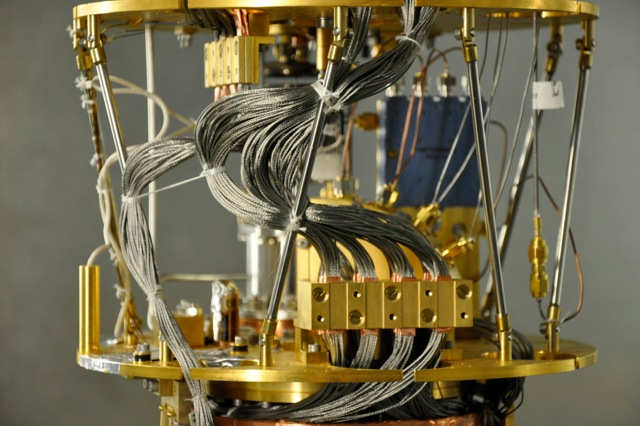
\includegraphics[width=\linewidth]{chapter1/quantum-computer-picture}
    \caption{Support structure for a D-WAVE quantum computer.}
    \label{fig:chapter1-quantum-computer-picture}
\end{marginfigure}

\footnote{\cite{Chapter1-quantum-computer-picture}}
In short, quantum computer can solve problems we can never solve with classical computer.
For example, there is an encryption algorithm we use everywhere, everyday, called RSA algorithm.
By using RSA algorithm, our passwords are encrypted during transmission and keep our money/data safe.
It is safe because it will take centuries for the most powerful super computer to decrypt the message encrypted by RSA.
But for quantum computer? This decryption process could be just a matter of seconds. 
What does that mean? If you have a quantum computer today, you would be able to hack almost all bank accounts on earth.
Of course, we don't want to build a quantum computer only good for hacking bank accounts, right?
There are a number of other applications like climate simulation, machine learning, material research, etc.
You already know how computers change the world.
Then just imagine the world will be changed again by quantum computers, and embrace the future!

\section{\textbf{How} can we try quantum computing?}
As of April 2018, there are a few options for us to write quantum programs on a simulated quantum computer.
Why simulated quantum computer? Because the real quantum computer doesn't exist yet!
Furthermore, using simulated quantum computer can get our hands dirty already.
The Q# language from Microsoft will be used as the main language for quantum programs throughout the book.

%----------------------------------------------------------------------------------------
%	CHAPTER 2
%----------------------------------------------------------------------------------------

\chapter{Chapter 2 Title}
\label{ch:2}

%----------------------------------------------------------------------------------------

\backmatter

%----------------------------------------------------------------------------------------
%	BIBLIOGRAPHY
%----------------------------------------------------------------------------------------

\bibliography{bibliography} % Use the bibliography.bib file for the bibliography
\bibliographystyle{plainnat} % Use the plainnat style of referencing

%----------------------------------------------------------------------------------------

\printindex % Print the index at the very end of the document

\end{document}